Одним из этапов проведения компьютерной экспертизы является анализ установленного программного обеспечения. Общеизвестно, что наличие единого реестра в системе, стало одной из особенностей операционной систем семейства Windows. В большинстве случаев, программы используют его в качестве хранения каких-либо данных.

Реестр Windows представляет собой иерархически построенную базу данных. На этапе загрузки операционная система собирает его из <<исходных>> файлов, разбросанных по своему дистрибутиву.

Целью работы за этот семестр стояло извлечь полезную информацию из реестра Windows, для достижения которой были выделены следующие задачи:

\begin{enumerate}
  \item исследовать механизм формирования реестра;
  \item написание программного модуля, способного извлекать информацию из реестра.
\end{enumerate}

\subsubsection{Исследование механизма формирования реестра}

Семестром ранее был установлен список исходных файлов реестра и было проведено первое знакомство с их структурой.

В ходе исследования одного из файлов было установлено, что он представляет собой <<чистый>> байтовый массив данных (рис.~\ref{lob_1:lob_1}). Встал вопрос о структуре данных в нем.

Компания Microsoft разрабатывает операционную систему Windows с конца прошлого века и, несмотря на <<закрытость>> исходного кода, время от времени выкладывает код отдельных ее модулей. \cite{registry} К сожалению, к ним не относится модуль реестра.

Из альтернативных источников можно получить лишь приблизительное представление внутренней структуре (рис.~\ref{lob_2:lob_2}). \cite{msdn}

К сожалению, из-за недостатка информации, придется на время отказаться от идеи разбора <<сырых>> файлов.

\begin{figure}[h!]
\center{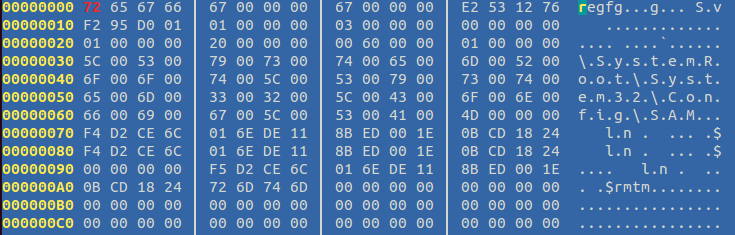
\includegraphics[width=0.9\linewidth]{lob_1}}
\caption{Файл SAM в HEX редакторе}
\label{lob_1:lob_1}
\end{figure} 

\begin{figure}[h!]
\center{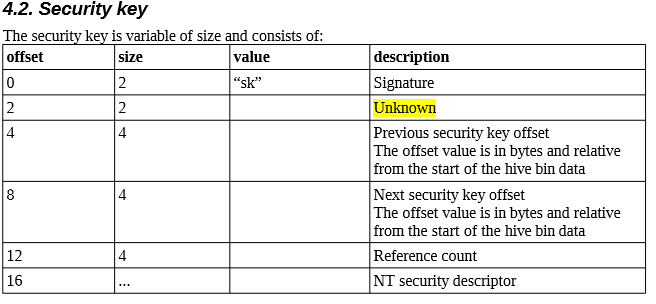
\includegraphics[width=0.9\linewidth]{lob_2}}
\caption{Пример описания одного из «простейших» блоков данных}
\label{lob_2:lob_2}
\end{figure} 

\subsubsection{Написание программного модуля, способного извлекать информацию из реестра}

С помощью встроенной в Windows утилиты regedit был сделан дамп всего древа реестра. Дальнейшая работа будет вестись с этим дампом.

Файл представляет из себя строковый массив с данными 2-х видов:

\begin{enumerate}
  \item описание ветви: [путь\_через\_узлы];
  \item описание данных: <<название поля>> = значение.
\end{enumerate}



\begin{figure}[h!]
\center{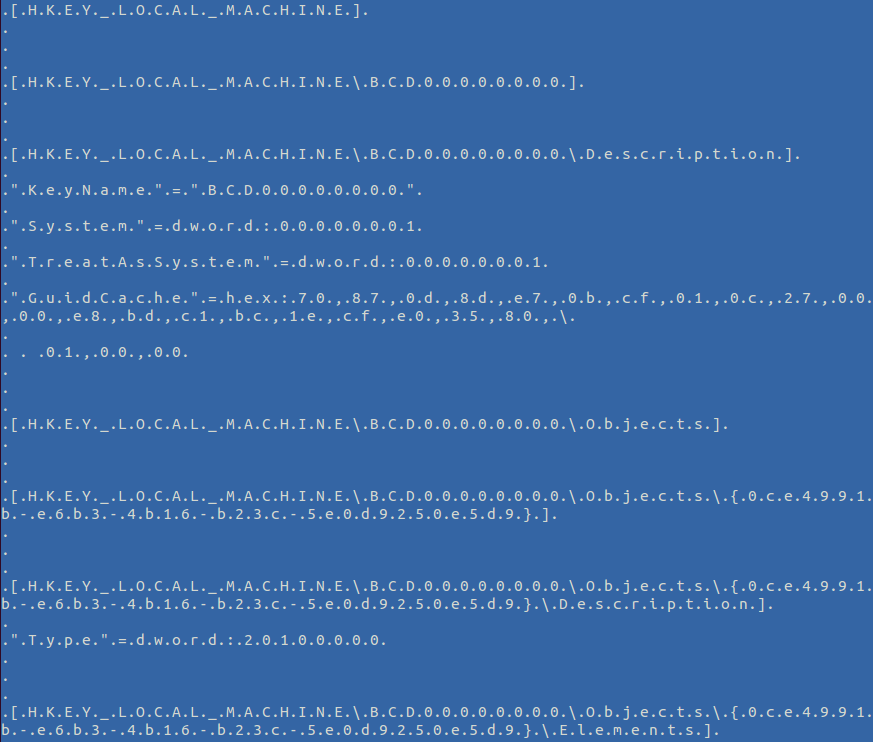
\includegraphics[width=0.9\linewidth]{lob_3}}
\caption{Внутренности .reg файла}
\label{lob_3:lob_3}
\end{figure} 

\begin{figure}[h!]
\center{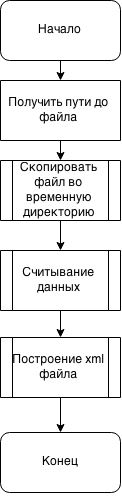
\includegraphics[width=0.2\linewidth]{lob_4}}
\caption{Блок-схема алгоритма работы модуля}
\label{lob_4:lob_4}
\end{figure} 

Считывание данных происходит построчно, рассмотрим в общем виде, как оно должно проходить (рис.~\ref{lob_5:lob_5}).

Пример работы программы представлен на рисунке~\ref{lob_6:lob_6}, результат работы программы --- на рисунке~\ref{lob_7:lob_7}.

\begin{figure}[h!]
\center{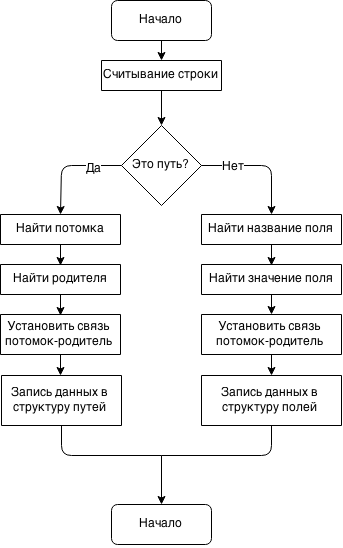
\includegraphics[width=0.4\linewidth]{lob_5}}
\caption{Функция разбора одной строки}
\label{lob_5:lob_5}
\end{figure} 

\begin{figure}[h!]
\center{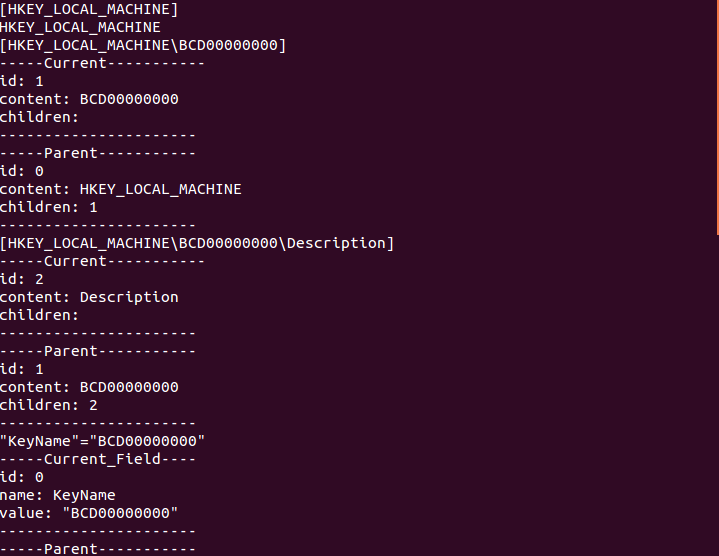
\includegraphics[width=0.7\linewidth]{lob_6}}
\caption{Пример работы программы}
\label{lob_6:lob_6}
\end{figure} 

\begin{figure}[h!]
\center{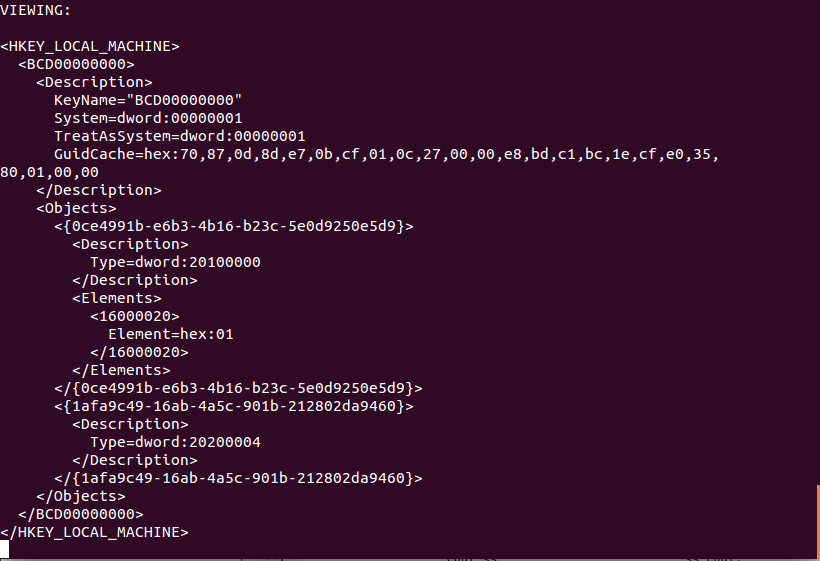
\includegraphics[width=0.7\linewidth]{lob_7}}
\caption{Результат работы программы}
\label{lob_7:lob_7}
\end{figure} 

\subsubsection{Результаты работы за семестр}

Результаты работы за текущий семестр:

\begin{enumerate}
  \item проведено доисследование структуры исходных файлов реестра;
  \item написан модуль получения информации из реестра windows. Информация берется из .reg файлов.
\end{enumerate}

Планы на будущее:

\begin{enumerate}
  \item дальнейший поиск описаний структура исходных файлов;
  \item по возможности, написание модуля извлечения информации из этих файлов.
\end{enumerate}

\clearpage






